%----------------------------------------------------------------------------------------
%	PACKAGES AND OTHER DOCUMENT CONFIGURATIONS
%----------------------------------------------------------------------------------------
\documentclass[12pt]{article}
\usepackage[english]{babel}
\usepackage[utf8x]{inputenc}
\usepackage{amsmath, amssymb}
\usepackage{graphicx}
\usepackage{caption}
\usepackage{float}
\usepackage{url}
\usepackage[colorinlistoftodos]{todonotes}
\usepackage{hyperref}
\usepackage[numbers]{natbib}
\usepackage{titletoc}
\usepackage{listings}
\usepackage{xcolor}
\usepackage{tcolorbox}
\usepackage{geometry}
\usepackage{tikz}
\usepackage{array}
\usetikzlibrary{positioning}
\geometry{
    a4paper,
    total={170mm,257mm},
    left=20mm,
    right=20mm,
    top=20mm,
    bottom=20mm,
}

\tcbset{
  mydefinition/.style={
    colback=violet!10,    % Couleur de fond
    colframe=violet,      % Couleur du cadre
    fonttitle=\bfseries,  % Style du titre
    coltitle=white,       % Couleur du titre
    boxrule=1mm,          % Épaisseur du cadre
    width=\textwidth,     % Largeur de la boîte
    sharp corners,        % Angles droits
    left=1mm, right=1mm,  % Marges internes
    top=1mm, bottom=1mm,  % Marges internes
  }
}

% Configuration des couleurs
\definecolor{codegreen}{rgb}{0,0.5,0}
\definecolor{codegray}{rgb}{0.5,0.5,0.5}
\definecolor{codepurple}{rgb}{0.58,0,0.82}
\definecolor{backcolour}{rgb}{0.95,0.95,0.92}
\definecolor{textcolor}{rgb}{0.33,0.33,0.33}

% Configuration de lstlisting
\lstset{
  backgroundcolor=\color{backcolour},
  commentstyle=\color{codegreen},
  keywordstyle=\color{magenta},
  numberstyle=\tiny\color{codegray},
  stringstyle=\color{codepurple},
  basicstyle=\footnotesize\color{textcolor},
  breakatwhitespace=false,
  breaklines=true,
  captionpos=b,
  keepspaces=true,
  numbers=left,
  numbersep=5pt,
  showspaces=false,
  showstringspaces=false,
  showtabs=false,
  tabsize=2
}
\newcommand{\subsubsubsectionbreak}{\par\addvspace{3.25ex plus 1ex minus .2ex}}
% Définition de la commande \touche
\newcommand{\touche}[1]{%
    \begin{tikzpicture}
        \pgfmathsetlengthmacro{\toucheboxwidth}{width("#1")+5pt} % Largeur de la boîte
        \draw[rounded corners=2pt, fill=black] (0,0) rectangle (\toucheboxwidth,0.5);
        \draw[rounded corners=1pt, fill=white] (0.05,0.05) rectangle (\toucheboxwidth-0.05,0.45);
        \node at (\toucheboxwidth/2,0.25) {#1};
    \end{tikzpicture}%
}
\newcommand{\toucheplus}{%
    \begin{tikzpicture}
        %\draw[rounded corners=2pt, fill=black] (0,0) rectangle (0.5,0.5);
        %\draw[rounded corners=1pt, fill=white] (0.05,0.05) rectangle (0.45,0.45);
        \node at (0.2,0.2) {+};
    \end{tikzpicture}%
}

\begin{document}
\begin{titlepage}
\newcommand{\HRule}{\rule{\linewidth}{0.5mm}} % Defines a new command for the horizontal lines, change thickness here
\center % Center everything on the page

%----------------------------------------------------------------------------------------
%	HEADING SECTIONS
%----------------------------------------------------------------------------------------
\textsc{\LARGE Ecole Supérieure d'Ingénieurs Léonard-de-Vinci}\\[1cm]

\includegraphics[scale=.4]{logo_esilv.png}\\[1cm]
\textsc{\Large Innovation In Finance}\\[0.5cm]
\textsc{\large Bonus Exercice 1}\\[0.5cm]
%----------------------------------------------------------------------------------------
%	TITLE SECTION
%----------------------------------------------------------------------------------------
\HRule \\[0.4cm]
{ \huge \bfseries Network analysis of CAC40 stocks}\\[0.4cm]
\HRule \\[0.5cm]
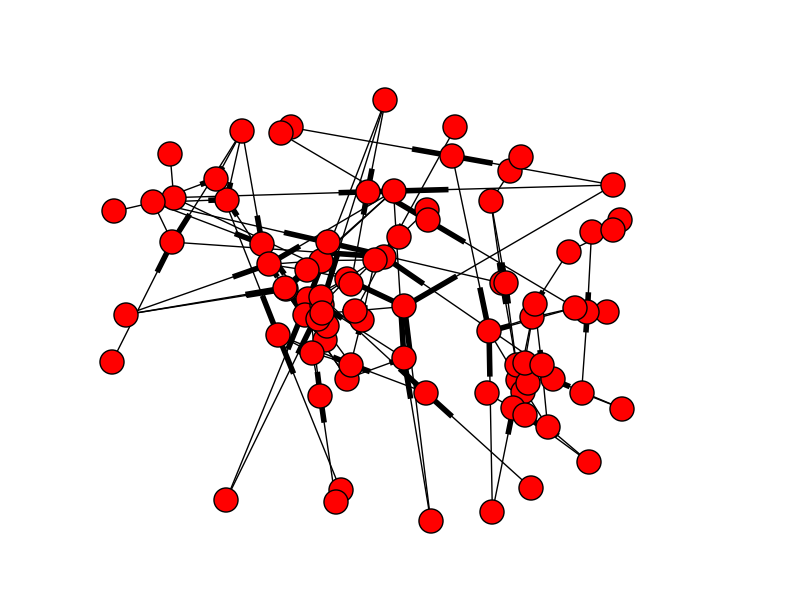
\includegraphics[scale=0.5]{network_stock_page_de_garde.png}\\
%----------------------------------------------------------------------------------------
%	AUTHOR SECTION
%----------------------------------------------------------------------------------------
Antoine \textsc{Buffandeau}\\
Charles \textsc{François}\\
Mathieu \textsc{Gourmelen}\\
%\Large \emph{Supervisors:}\\
 \textsc{}
\\[1cm]
%----------------------------------------------------------------------------------------
%	DATE SECTION
%----------------------------------------------------------------------------------------
{\large \today} % Date, change the \today to a set date if you want to be precise
\vfill
\end{titlepage}
%----------------------------------------------------------------------------------------
%	TABLE OF CONTENTS SECTION
%----------------------------------------------------------------------------------------
\tableofcontents
%----------------------------------------------------------------------------------------
%	INTRODUCTION SECTION
%----------------------------------------------------------------------------------------
\hypertarget{sec:part1}{}
\section{Introduction}
This report explores the structure of a stock correlation network created from a dataset comprising the evolution of stock prices for companies listed in the CAC40 between 2018 and 2023. The dataset provides pairwise correlations between these stocks, which are used to construct a network with connections based on specific correlation thresholds. By applying network science techniques, this study investigates connectivity, community structures, and core-periphery roles within the network.
\begin{figure}[h!]
  \centering
  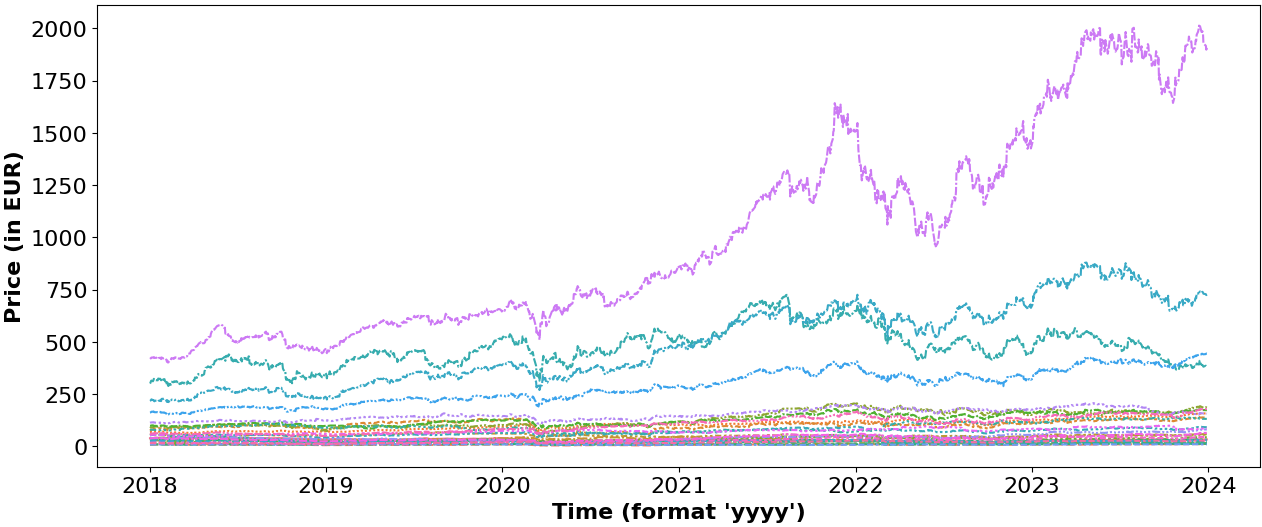
\includegraphics[width=\textwidth]{close_price_index_cac40_stocks.png}
  \caption{Dataset overview, daily closing prices of CAC 40 index stocks}
  \label{fig:stock_close_price}
\end{figure}
%----------------------------------------------------------------------------------------
%	SECTION 1 
%----------------------------------------------------------------------------------------
\section{Dataset and Threshold-Based Network Construction}
We utilized a dataset detailing daily closing prices and derived pairwise correlations of CAC40 stocks. Networks were constructed at three correlation thresholds (0.3, 0.5, and 0.7) to manipulate the density and connectivity of the network. Each threshold was selected to demonstrate how varying levels of correlation strength influence the overall network structure, from dense (low threshold) to sparse (high threshold).
\clearpage

\begin{figure}[h!]
  \centering
  \begin{minipage}[b]{0.32\textwidth}
      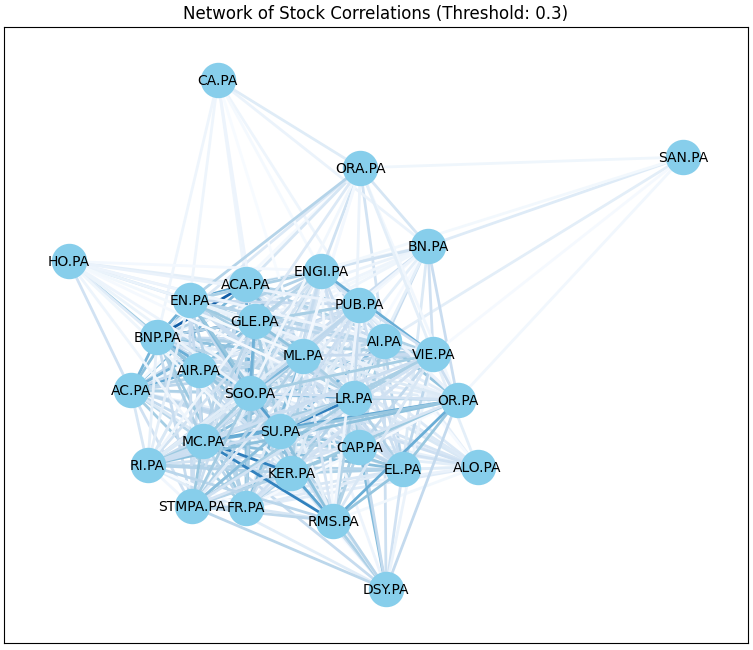
\includegraphics[width=\textwidth]{2D_network_stock_corr3.png}
      \caption{Threshold 0.3}
      \label{fig:threshold03}
  \end{minipage}
  \hfill
  \begin{minipage}[b]{0.32\textwidth}
      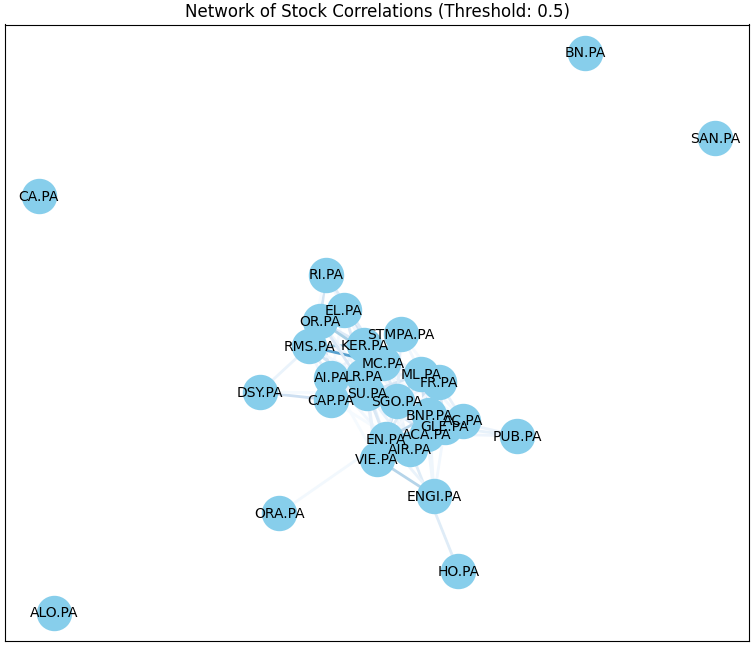
\includegraphics[width=\textwidth]{2D_network_stock_corr5.png}
      \caption{Threshold 0.5}
      \label{fig:threshold05}
  \end{minipage}
  \hfill
  \begin{minipage}[b]{0.32\textwidth}
      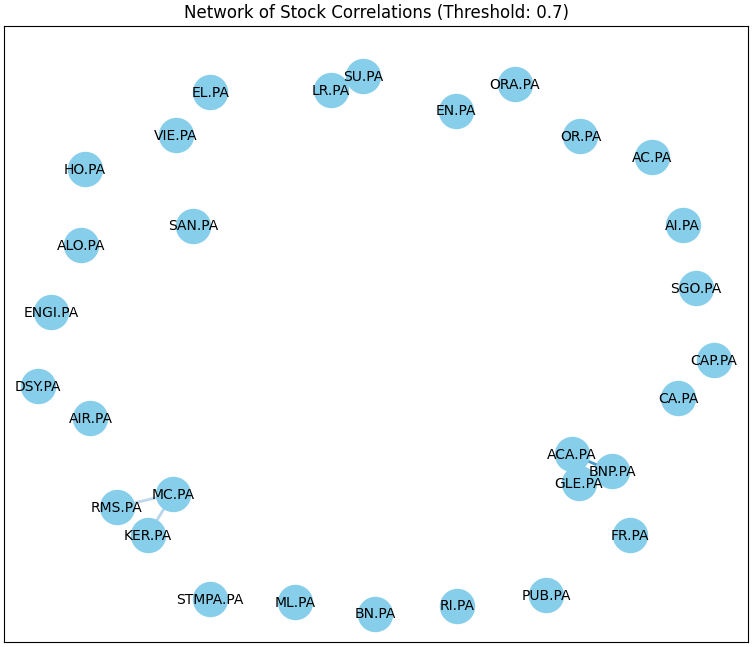
\includegraphics[width=\textwidth]{2D_network_stock_corr7.png}
      \caption{Threshold 0.7}
      \label{fig:threshold07}
  \end{minipage}
  %\caption{Network of Stock Correlations at Different Thresholds}
  \label{fig:stock_networks}
\end{figure}

•	Threshold 0.3 : this network graph demonstrates a dense connectivity pattern among CAC40 stocks. A lower threshold of 0.3 includes weaker correlations, resulting in a more interconnected network where most stocks are directly or indirectly linked to multiple others, suggesting a market where stocks are broadly responsive to shared economic factors.

•	Threshold 0.5 : at a moderate threshold of 0.5, the network shows reduced density, indicating that only medium to strong correlations are considered significant enough to form connections. This results in a sparser graph where only genuinely correlated stocks are connected, eliminating weaker, less significant relationships. 

•	Threshold 0.7 : with the highest threshold set at 0.7, the graph presents a very sparse network with few connections, highlighting only the strongest correlations among stocks. This sparse connectivity implies a highly selective relationship, where only the most robust correlations persist, suggesting that these connections may represent fundamental structural ties within the market.

\section{Step-by-Step Analysis}

\subsection{Step 1: Network Metrics}
Key metrics including average degree, density, transitivity, and assortativity were calculated for each thresholded network.

\begin{itemize}
    \item \textbf{The Average Degree}, that is to say the average number of connections (edges) per node (stock) in the network, it reflects the typical number of direct relationships each stock has with others in the network. In our case, the average degree decreases with increasing thresholds, indicating fewer connections as weaker correlations are removed.
    \begin{figure}[H]
        \centering
        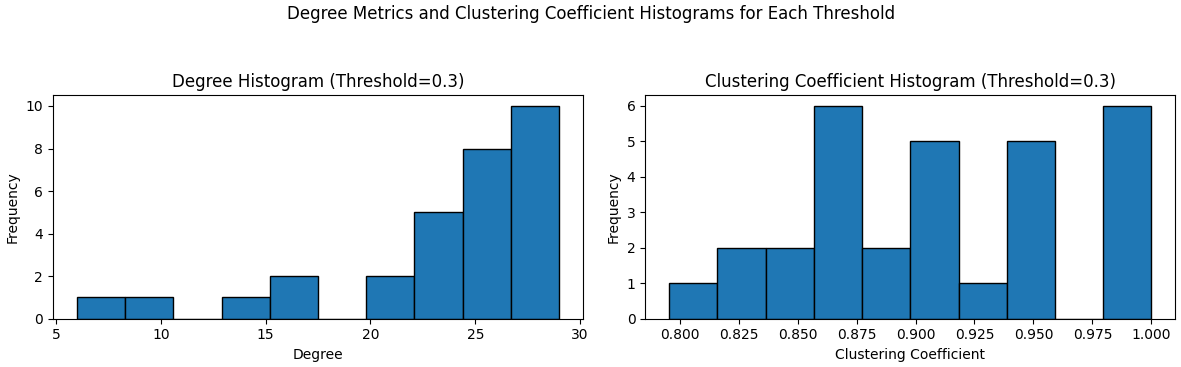
\includegraphics[width=\textwidth]{degree_cluster_coeff_network_stock_corr3.png}
        %\caption{Degree and Clustering Coefficient Histograms for Threshold = 0.3}
        \label{fig:degree_clustering_03}
    \end{figure}
    \begin{figure}[H]
        \centering
        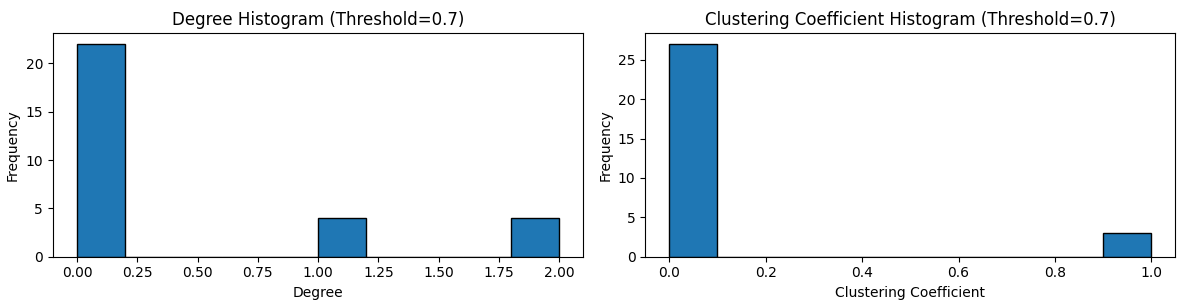
\includegraphics[width=\textwidth]{degree_cluster_coeff_network_stock_corr7.png}
        %\caption{Degree and Clustering Coefficient Histograms for Threshold = 0.7}
        \label{fig:degree_clustering_07}
    \end{figure}
    \item \textbf{The Density} measures the proportion of potential connections in the network that are actual connections. High density indicates a closely knit network, where many possible pairs of stocks are directly connected.  Here, the density drops significantly from 0.8092 at 0.3 to 0.0138 at 0.7, confirming that the network becomes sparser.
    \item \textbf{The Transitivity} reflects the likelihood that the neighbors (connected nodes) of a node are also connected to each other. A high transitivity indicates that the network has many tightly knit groups or clusters. In our study, the transitivity reveals high clustering at lower thresholds, remaining elevated at 0.3 but diminishing at 0.5 and 0.7.
    \item \textbf{The Assortativity} generally indicates the tendency of nodes to connect with other nodes that are similar in some way, in this case, degree. Positive assortativity suggests that stocks tend to connect with others that have a similar number of connections, whereas negative assortativity indicates that stocks tend to connect with others that have different numbers of connections. Here, we have a negative assortativity at lower thresholds, indicating a hub-like structure, and turns positive at 0.7, suggesting that remaining connections form among degree-similar nodes.
\end{itemize}

\begin{table}[H]
    \centering
    \begin{tabular}{|c|c|c|c|c|}
        \hline
        Threshold & Avg Degree & Density & Transitivity & Assortativity \\
        \hline
        0.3 & 23.47 & 0.8092 & 0.8957 & -0.1183 \\
        0.5 & 8.73 & 0.3011 & 0.6573 & -0.1053 \\
        0.7 & 0.4 & 0.0138 & 0.7500 & 0.2500 \\
        \hline
    \end{tabular}
    \caption{Network Metrics at Different Thresholds.}
\end{table}

\subsection{Step 2: Centrality Measures}
Centrality measures are crucial in network analysis as they help identify the most influential nodes within a network. In the context of a stock correlation network, these measures can reveal which stocks are central in terms of market movements and potential influence on other stocks. Here, we calculated four different types of centrality measures:\\

- Degree Centrality: counts the number of direct connections a node has. 

- Closeness Centrality: measures how quickly information from a node can reach all other nodes in the network through its direct and indirect connections. 

- Betweenness Centrality: quantifies how often a node appears on the shortest paths between other nodes in the network. 

- Eigenvector Centrality: a measure of a node's influence based on the quality, not just quantity, of its connections. \\

By analyzing these centrality measures, we can identify which stocks are likely to be key players in the CAC40 index, influencing overall market trends and stability. For instance:

•	At lower thresholds (0.3), where the network is denser, centrality might be more distributed, indicating a market environment where many stocks are interconnected and collectively influence the market.

•	At higher thresholds (0.7), centrality may concentrate in fewer stocks, highlighting those that maintain strong correlations despite the stringent threshold. These stocks could be crucial for understanding core market movements and strategic investment decisions.

\subsection{Step 3: Comparison with Network Models}
The constructed stock networks were compared to Erdős-Rényi and Barabási-Albert models:
\begin{itemize}
    \item \textbf{Erdős-Rényi Model} displayed low clustering and random connections, lacking the structural properties of the stock network.
    \item \textbf{Barabási-Albert Model} created a hub structure, forming a few highly connected nodes. While closer to the stock network, it did not fully capture the clustering observed in the data.
\end{itemize}

\begin{table}[H]
    \centering
    \begin{tabular}{|c|c|c|c|}
        \hline
        Model & Threshold & Transitivity & Assortativity \\
        \hline
        Stock Network & 0.3 & 0.8957 & -0.1183 \\
        Erdős-Rényi & 0.3 & 0.7970 & -0.0899 \\
        Barabási-Albert & 0.3 & 0.5488 & -0.3182 \\
        Stock Network & 0.7 & 0.7500 & 0.2500 \\
        Erdős-Rényi & 0.7 & 0.0000 & -0.5000 \\
        Barabási-Albert & 0.7 & 0.0000 & -0.3443 \\
        \hline
    \end{tabular}
    \caption{Comparison of Network Transitivity and Assortativity.}
\end{table}

\subsection{Step 4: Community Detection (Louvain Method)}
The Louvain method was applied to detect communities within each thresholded network. At lower thresholds, stocks naturally formed larger, densely connected communities, likely reflecting sector-based groupings or interrelated stocks. Modularity, which measures the strength of community division, was highest at threshold 0.3, indicating well-defined clusters.
\begin{figure}[H]
    \centering
    \begin{minipage}[b]{0.45\textwidth}
        \centering
        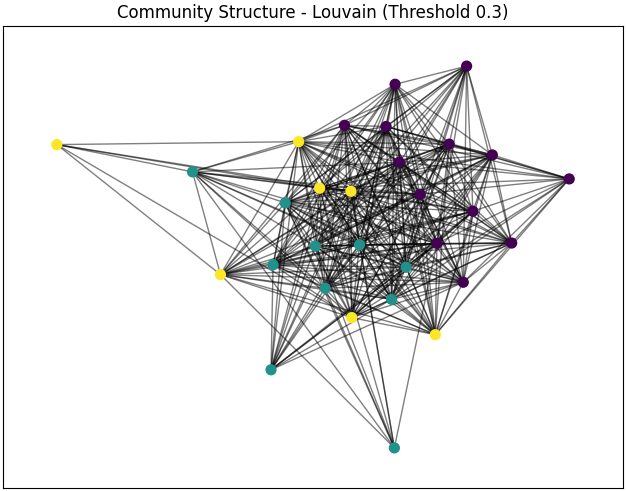
\includegraphics[width=\textwidth]{louvain_network_stock_corr3.png}
        %\caption{Community Structure - Louvain (Threshold 0.3)}
        \label{fig:louvain_03}
    \end{minipage}
    \hfill
    \begin{minipage}[b]{0.45\textwidth}
        \centering
        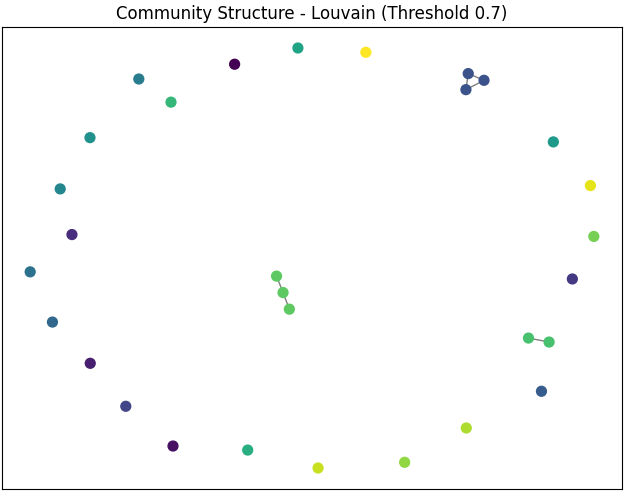
\includegraphics[width=\textwidth]{louvain_network_stock_corr7.png}
        %\caption{Community Structure - Louvain (Threshold 0.7)}
        \label{fig:louvain_07}
    \end{minipage}
    \caption{Comparison of Community Structures at Thresholds 0.3 and 0.7}
    \label{fig:community_structures}
\end{figure}
\subsection{Step 5: Core-Periphery Analysis}
Using k-core decomposition, core-periphery structure was analyzed for each threshold:
\begin{itemize}
    \item \textbf{Core Stocks}: At threshold 0.3, multiple stocks formed the core, indicating strong interconnectedness within the network.
    \item \textbf{Periphery Stocks}: At threshold 0.7, only a small core remained, with most stocks in the periphery, showing a distinct separation between central and isolated stocks.
\end{itemize}

\section{Conclusion}

Our analysis underscores that the CAC40 stock network differs significantly from random and scale-free models, exhibiting unique clustering, centrality, and core-periphery structures. As thresholds increase, connectivity decreases, isolating clusters of highly correlated stocks and leaving only a few central nodes. The results highlight the stock network’s natural clustering and centrality patterns, which suggest inherent relationships that might align with sectors or market dynamics.

%----------------------------------------------------------------------------------------
%	PART REFERENCES
%---------------------------------------------------------------------------------------
%\part{Références}
%\cite{EBA_website}
%\bibliographystyle{IEEEtran}
%\bibliography{ref_RS.bib}
%----------------------------------------------------------------------------------------
%	ENDING SECTION
%----------------------------------------------------------------------------------------
\end{document}